\section{Repository-Grounded Results}

The article now includes a compact but nontrivial empirical slice drawn from executable tutoring architectures already present in the repository. The evidence is intentionally narrower than a full benchmark study: we analyze aligned 30-example snapshots rather than complete benchmark passes. Even so, those snapshots are useful because they compare multiple architectural families under matched sample counts and expose how benchmark regime changes which design looks strongest.

\subsection{Setup summary}

The repository currently supports EduBench and TutorEval through a shared dataset registry. For the runs summarized here, the comparison covers four implemented families: classical RAG, hybrid-fast agentic RAG, non-RAG multi-agent tutoring, and a single-agent no-RAG baseline. These comparisons should be read as repository-grounded directional evidence rather than as final leaderboard claims. The main value of the snapshots is not absolute score reporting, but architectural contrast under the same local execution stack.

\subsection{Published benchmark context}

Table~\ref{tab:public} gives published benchmark context from official sources. The purpose is to show that both EduBench and TutorEval are meaningful evaluation targets with established public baselines. The numbers are not directly comparable to the repository logs because the evaluation protocols differ.

\begin{table}[t]
\caption{Published benchmark context from official sources. These numbers provide difficulty context only and are not directly comparable to the repository-grounded ablations in Table~\ref{tab:main}.}
\label{tab:public}
\centering
\scriptsize
\begin{tabular}{p{1.25cm}p{3.15cm}p{1.85cm}}
\toprule
Benchmark & Reported reference result & Source \\
\midrule
EduBench & R1: 8.71; Qwen: 8.06 & \cite{xu2025edubench} \\
TutorEval & GPT-4: 85.2 / 86.1; Llama-3-70B: 71.3 / 78.3 & \cite{chevalier2024sciencetutors,lmsciencetutorrepo} \\
\bottomrule
\end{tabular}
\end{table}

\subsection{Architecture comparison on aligned snapshots}

Table~\ref{tab:main} reports the aligned repository snapshots. The pattern is deliberately mixed. On EduBench, the non-RAG multi-agent route produces the strongest rubric coverage and score alignment in the aligned snapshot while also being the fastest configuration shown. On TutorEval, which rewards evidence-grounded tutoring over long science passages more strongly, the hybrid-fast route produces the best token F1, rubric coverage, and grounded overlap while remaining substantially faster than classical RAG. This is the core architectural result of the current paper: the preferred tutoring architecture shifts with the benchmark regime.

\begin{table*}[t]
\caption{Repository-grounded architecture comparison using aligned 30-example snapshots from \texttt{web/data/session\_summary.json}. Metrics are shown only where a benchmark exposes the needed supervision signal; higher is better except latency.}
\label{tab:main}
\centering
\scriptsize
\begin{tabular}{llcccc}
\toprule
Dataset & Architecture & Token F1 / Overlap & Rubric Coverage & Score Align / Grounded Overlap & Latency (ms) \\
\midrule
\multirow{4}{*}{EduBench}
& Classical RAG & 0.0000 & 0.7607 & 0.0333 / 0.3129 & 39{,}494.2 \\
& Hybrid-fast & 0.0000 & 0.8829 & 0.0774 / 0.0000 & 33{,}941.5 \\
& Non-RAG multi-agent & 0.0000 & \textbf{0.9116} & \textbf{0.1628} / 0.0000 & \textbf{33{,}692.3} \\
& Single-agent no-RAG & 0.0000 & 0.7645 & 0.1355 / 0.0000 & 36{,}439.0 \\
\midrule
\multirow{4}{*}{TutorEval}
& Classical RAG & 0.0622 & 0.9333 & 0.0000 / 0.2668 & 47{,}197.3 \\
& Hybrid-fast & \textbf{0.0642} & \textbf{0.9833} & 0.0000 / \textbf{0.2883} & 35{,}655.4 \\
& Non-RAG multi-agent & 0.0533 & 0.9722 & 0.0000 / 0.0000 & \textbf{35{,}071.7} \\
& Single-agent no-RAG & 0.0481 & 0.9500 & 0.0000 / 0.0000 & 49{,}808.7 \\
\bottomrule
\end{tabular}
\end{table*}

\subsection{Quality--latency frontier}

Figure~\ref{fig:tradeoff} visualizes the same evidence as a quality--latency trade-off. The plot makes the article's central systems point easier to see at a glance. The Pareto-efficient region is not occupied by one fixed family across both datasets. Instead, different benchmark demands favor different tutoring architectures.

\begin{figure*}[t]
\centering
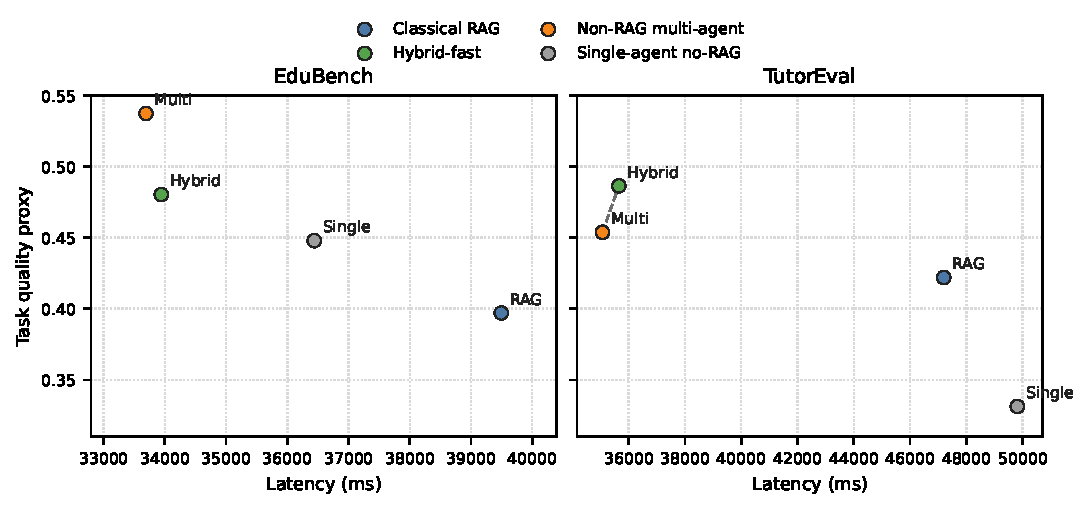
\includegraphics[width=0.88\textwidth]{build-artifacts/tradeoff_quality_latency.pdf}
\caption{Quality--latency trade-off from the aligned 30-example snapshots in Table~\ref{tab:main}. The preferred architecture changes by benchmark regime rather than remaining fixed.}
\label{fig:tradeoff}
\end{figure*}

\subsection{Interpretation}

The article-level takeaway is disciplined rather than universal. The repository snapshots do not show that classical RAG fails everywhere, nor do they show that non-RAG multi-agent systems dominate by default. They show something more useful for system design: once educational quality depends on tutoring-specific coordination, a fixed retrieve-then-generate controller is no longer globally dominant. Coordination-heavy workloads can favor non-RAG or hybrid routes, while evidence-grounded tutoring still benefits from retrieval when the system can invoke it conditionally.
